\chapter{Листинг программы}

На листинге \ref{lst3} показан код программы, выводящий агрумент с результатами работы методов, которые необходимо было реализовать по условию лабораторной.

\begin{lstlisting}[caption=код программы, label=lst1]
using System;
using System.Collections.Generic;
using System.Linq;
using System.Text;
using System.Threading.Tasks;

namespace lab2_modeling
{
    class Methods
    {
        public Methods()
        {
            fillData();
        }

        private double[,] ItK = {{0.5, 6700, 0.5},
                                {1, 6790, 0.55},
                                {5, 7150, 1.7},
                                {10, 7270, 3},
                                {50, 8010, 11},
                                {200, 9185, 32},
                                {400, 10010, 40},
                                {800, 11140, 41},
                                {1200, 12010, 39} };

        private double[,] Tsigma = {{4000, 0.031},
                                    {5000, 0.27},
                                    {6000, 2.05},
                                    {7000, 6.06},
                                    {8000, 12.0},
                                    {9000, 19.9},
                                    {10000, 29.6},
                                    {11000, 41.1},
                                    {12000, 54.1},
                                    {13000, 67.7},
                                    {14000, 81.5}};

        
        private static List<double>[] createGraph(int n = 2)
        {
            var graph = new List<double>[n];
            for (int i = 0; i < n; i++)
            {
                graph[i] = new List<double>();
            }
            return graph;
        }

        public List<double>[] graph1 = createGraph(2);
        public List<double>[] graph2 = createGraph(2);
        public List<double>[] graph3 = createGraph(2);
        public List<double>[] graph4 = createGraph(2);
        public List<double>[] graph5 = createGraph(2);

        private Dictionary<string, double> data = new Dictionary<string, double>();

        private void fillData()
        {
            data.Add("R", 0.35);
            data.Add("Le", 12);
            data.Add("Lk", 0.000187);
            data.Add("Ck", 0.000268);
            data.Add("Rk", 0.25);
            data.Add("Uc0", 1400);
            data.Add("I0", 0.5);
            data.Add("Tw", 2000);
            data.Add("Tbegin", 0);
            data.Add("Tend", 0.0006);
            data.Add("Tstep", 1e-6);
        }

        private double interpolate(double[,] table, double xValue, int xIndex, int yIndex)
        {
            bool interpolateIndexFound = false;
            double x1 = 0;
            double x2 = 0;
            double y1 = 0;
            double y2 = 0;
            double yResult = 0;
            int len = table.Length;
            if (len == 22)
                len = 11;
            else
                len = 9;

            for (int i = 0; i < len - 1; i++)
            {
                if (table[i,xIndex] <= xValue && xValue <= table[i + 1, xIndex])
                {
                    y1 = table[i, yIndex];
                    y2 = table[i + 1, yIndex];
                    x1 = table[i, xIndex];
                    x2 = table[i + 1, xIndex];
                    interpolateIndexFound = true;
                }
            }
            if (interpolateIndexFound)
            { 
                yResult = y1 + ((xValue - x1) / (x2 - x1)) * (y2 - y1); 
            }
            else
            {
                if (xValue < table[0, xIndex])
                    yResult = table[0, yIndex];
                if (xValue > table[len - 1, xIndex])
                    yResult = table[len - 1, yIndex];
            }

            return yResult;
        }


        private double integrateSimpson(double I)
        {
            double n = 40;
            double begin = 0;
            double end = 1;
            double width = (end - begin) / n;
            double result = 0;
            double x1, x2;
            for (double step = 0; step < n; step++)
            {
                x1 = begin + step * width;
                x2 = begin + (step + 1) * width;
                result += (x2 - x1) / 6.0 * (sigmaFunc(I, x1) + 4.0 * sigmaFunc(I, 0.5 * (x1 + x2)) + sigmaFunc(I, x2));
            }
            return result;
        }

        private double calculateRp(double I)
        {
            double R = data["R"];
            double integral = integrateSimpson(I);
            return data["Le"] / (2 * Math.PI * R * R * integral);
        }

        private double f_PHI(double t, double I, double U)
        {
            return -1 / data["Ck"] * I;
        }

        private double getTz(double T0, double m, double r)
        {
            double z = r;
            return (data["Tw"] - T0) * Math.Pow(z, m) + T0;
        }

        private double sigmaFunc(double I, double z)
        {
            double m = interpolate(ItK, I, 0, 2);
            double T0 = interpolate(ItK, I, 0, 1);
            double Tz = getTz(T0, m, z);
            double sigma = interpolate(Tsigma, Tz, 0, 1);
            return z * sigma;
        }

        private double functionF_4(double t, double I, double U)
        {
            double Rp = calculateRp(I);
            graph3[0].Add(t);
            graph3[1].Add(Rp);
            graph4[0].Add(t);
            graph4[1].Add(I * Rp);
            return (U - (data["Rk"] + Rp) * I) / data["Lk"];
        }

        private double[] Runge4(double xn, double yn, double zn, double hn)
        {
            double[] result = new double[2];

            double hn2 = hn / 2;
            double k1 = hn * functionF_4(xn, yn, zn);
            double q1 = hn * f_PHI(xn, yn, zn);

            double k2 = hn * functionF_4(xn + hn2, yn + k1 / 2, zn + q1 / 2);
            double q2 = hn * f_PHI(xn + hn2, yn + k1 / 2, zn + q1 / 2);

            double k3 = hn * functionF_4(xn + hn2, yn + k2 / 2, zn + q2 / 2);
            double q3 = hn * f_PHI(xn + hn2, yn + k2 / 2, zn + q2 / 2);

            double k4 = hn * functionF_4(xn + hn, yn + k3, zn + q3);
            double q4 = hn * f_PHI(xn + hn, yn + k3, zn + q3);

            double yn_1 = yn + (k1 + 2 * k2 + 2 * k3 + k4) / 6;
            double zn_1 = zn + (q1 + 2 * q2 + 2 * q3 + q4) / 6;

            result[0] = yn_1;
            result[1] = zn_1;
            return result;
        }

        public void beginCalculations()
        {
            double t = data["Tbegin"];
            double tmax = data["Tend"];
            double I = data["I0"];
            double Uc = data["Uc0"];
            double hn = data["Tstep"];
            for (double i = t; i < tmax + hn; i += hn)
            {
                graph1[0].Add(i);
                graph1[1].Add(I);
                graph2[0].Add(i);
                graph2[1].Add(Uc);
                graph5[0].Add(i);
                graph5[1].Add(interpolate(ItK, I, 0, 1));
                var result = Runge4(i, I, Uc, hn);
                I = result[0];
                Uc =result[1];
            }
        }
    }

}
\end{lstlisting}

\hspace{0cm} \textbf{Результат работы программы:}

На рисунках \ref{fig:fig1} - \ref{fig:fig5} графики зависимости от времени импульса $t: I(t),U(t),R_p(t),I(t)*R_p(t),T_0(t)$ при заданных в условиях параметрах разрядного контура.

\begin{figure}[ht!]
  \centering
  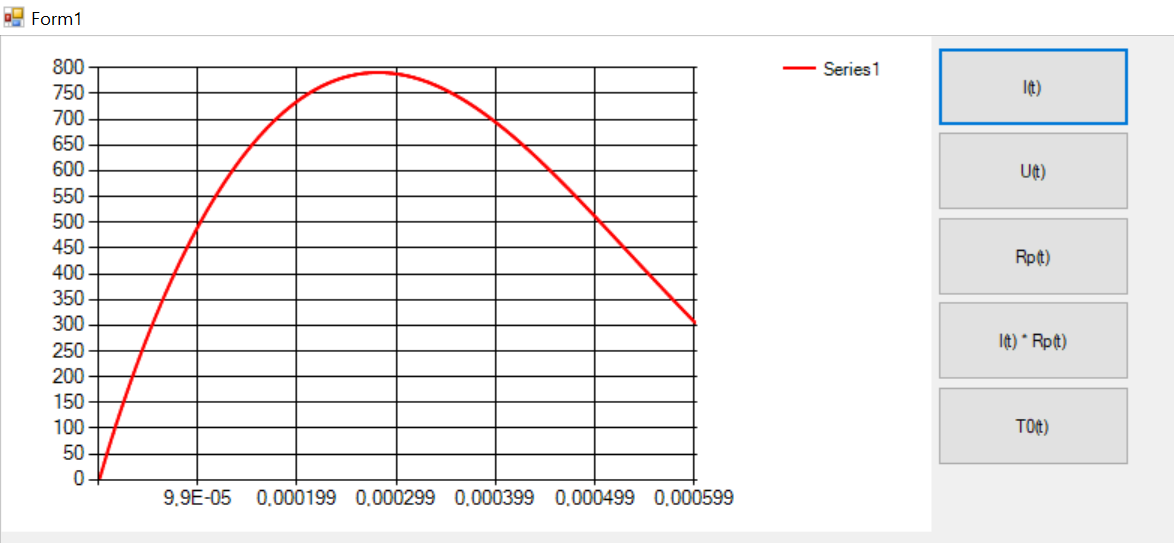
\includegraphics[scale=0.8]{img/I(t).png}
  \caption{график $I(t)$}
  \label{fig:fig1}
\end{figure}

\newpage

\begin{figure}[ht!]
  \centering
  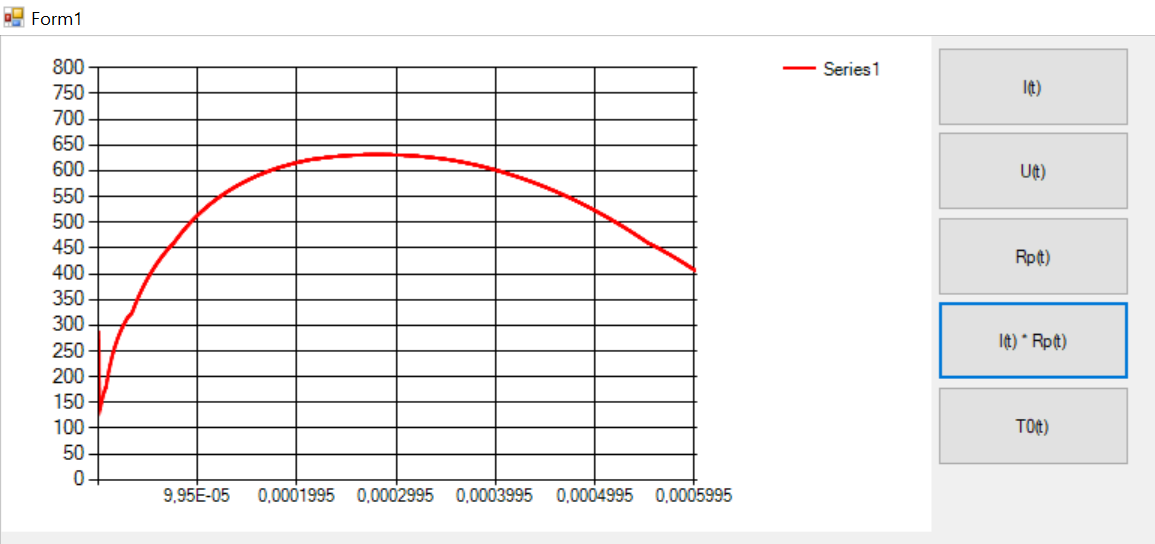
\includegraphics[scale=0.8]{img/I(t)Rp(t).png}
  \caption{график $I(t)*R_p(t)$}
  \label{fig:fig2}
\end{figure}

\begin{figure}[ht!]
  \centering
  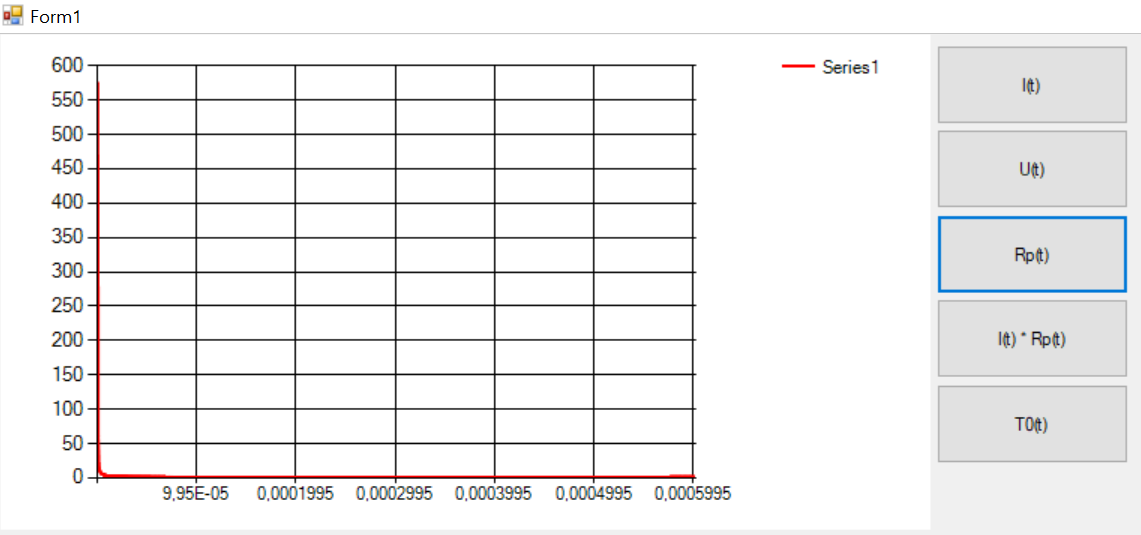
\includegraphics[scale=0.8]{img/Rp(t).png}
  \caption{график $R_p(t)$}
  \label{fig:fig3}
\end{figure}

\newpage

\begin{figure}[ht!]
  \centering
  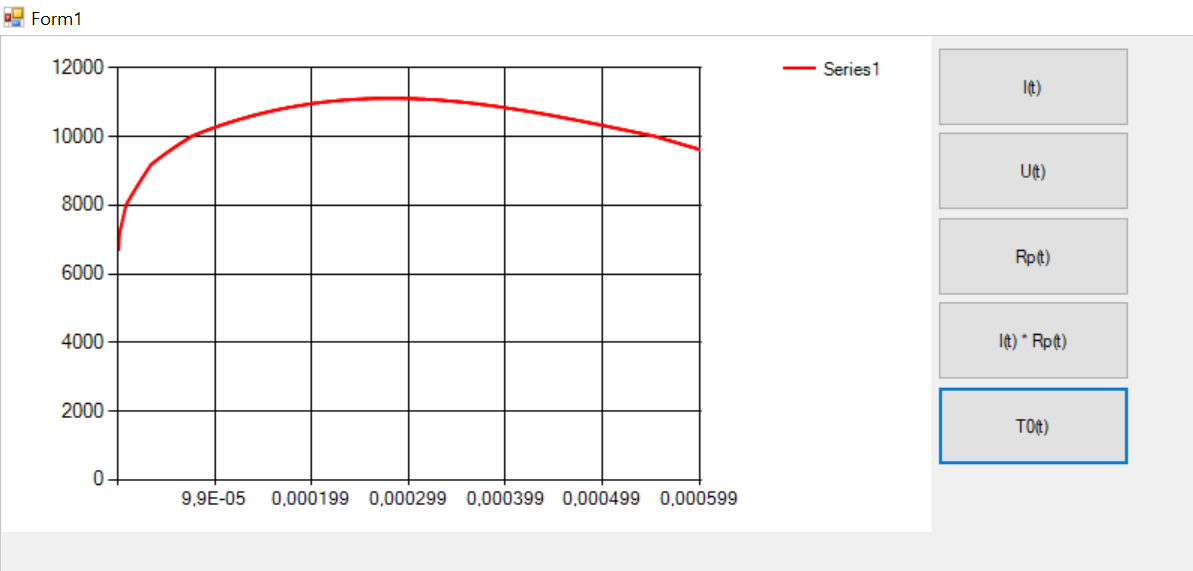
\includegraphics[scale=0.8]{img/T0(t).png}
  \caption{график $T_0(t)$}
  \label{fig:fig4}
\end{figure}

\begin{figure}[ht!]
  \centering
  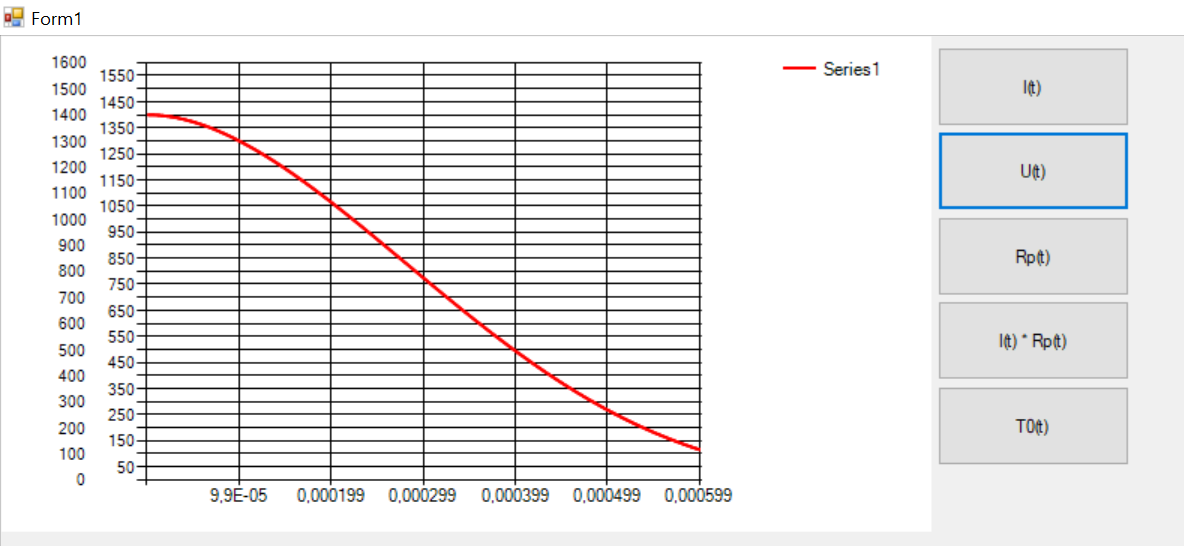
\includegraphics[scale=0.8]{img/U(t).png}
  \caption{график $U(t)$}
  \label{fig:fig5}
\end{figure}

\newpage

Графики зависимостей $I(t),U(t),R_p(t),I(t)*R_p(t)$ при $R_k+R_p=0$ приведены на рисунке \ref{fig:fig6}:

\begin{figure}[H]
\begin{minipage}[h]{0.47\linewidth}
\center{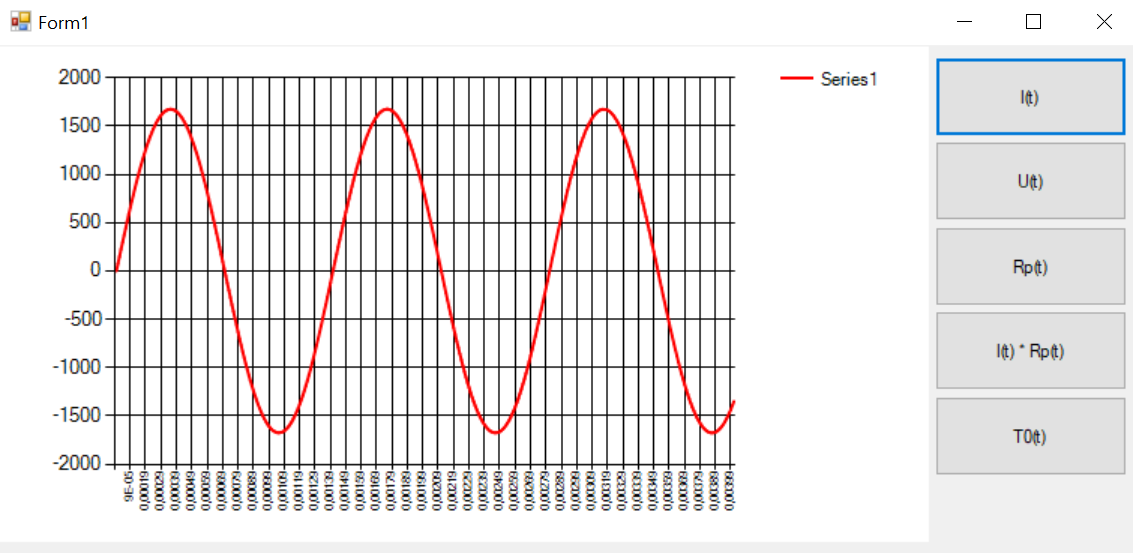
\includegraphics[width=1\linewidth]{img/I(t)RkRp0.png}} a) \\
\end{minipage}
\hfill
\begin{minipage}[h]{0.47\linewidth}
\center{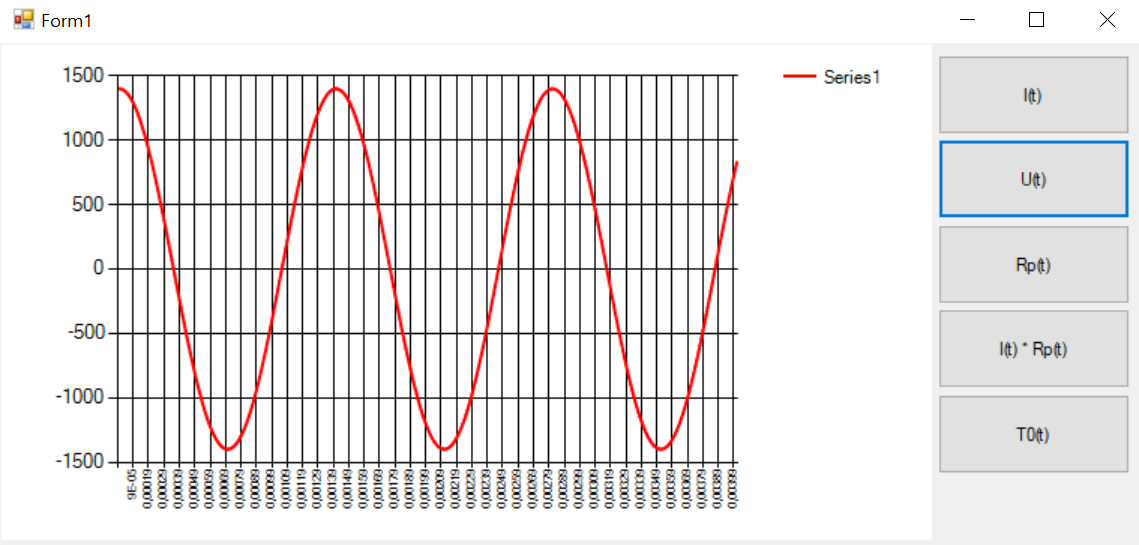
\includegraphics[width=1\linewidth]{img/U(t)RkRp0.png}} \\b)
\end{minipage}
\vfill
\begin{minipage}[h]{0.47\linewidth}
\center{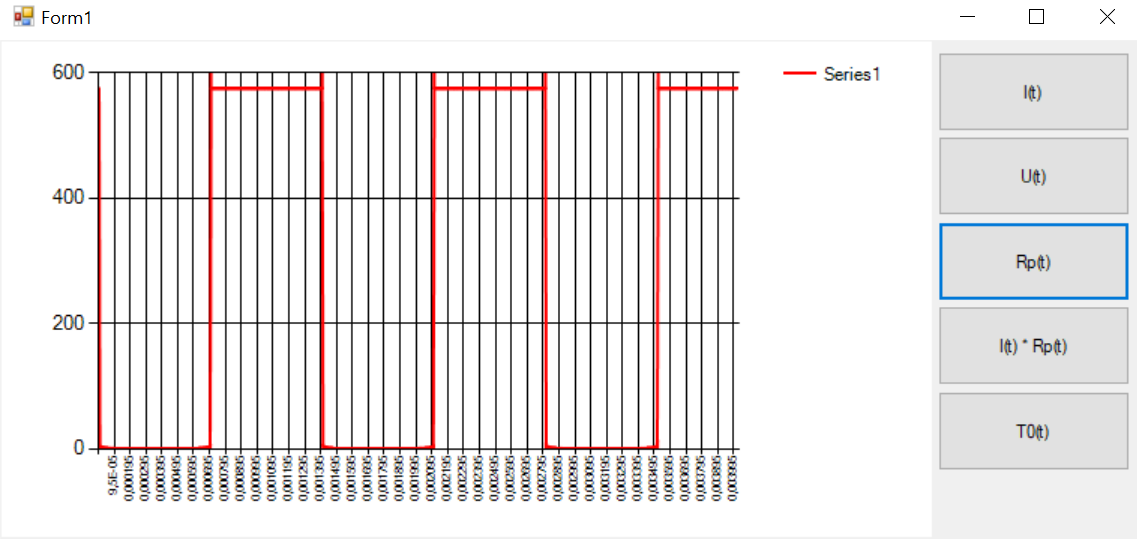
\includegraphics[width=1\linewidth]{img/Rp(t)RkRp0.png}} c) \\
\end{minipage}
\hfill
\begin{minipage}[h]{0.47\linewidth}
\center{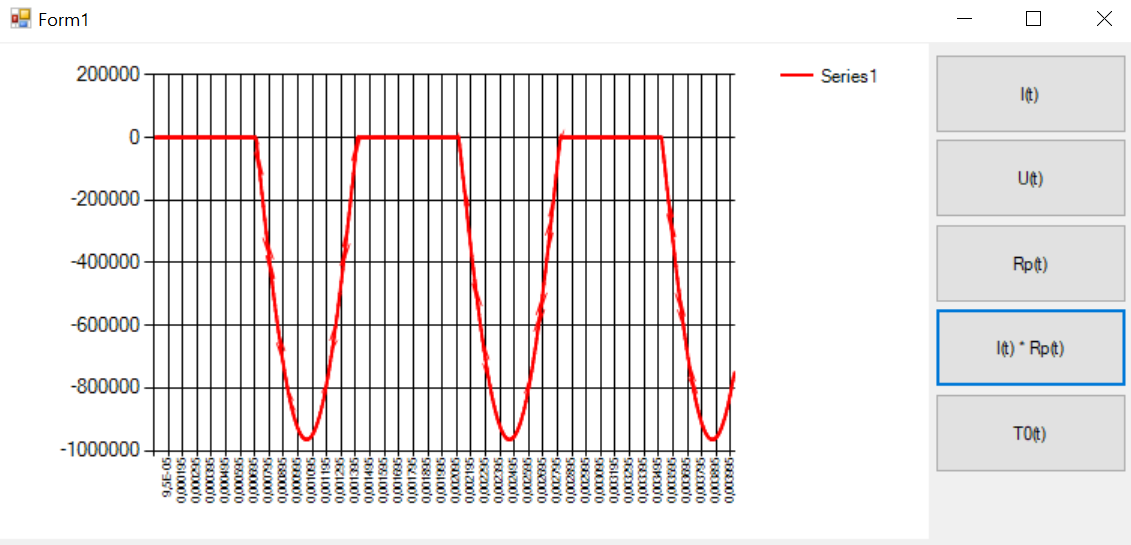
\includegraphics[width=1\linewidth]{img/I(t)Rp(t)RkRp0.png}} d) \\
\end{minipage}
\caption{Графики: a) I(t), b)
U(t), c) $R_p(t)$, d) $I(t)*R_p(t)$.}
\label{fig:fig6}
\end{figure}

Графики зависимости $I(t),U(t),R_p(t),I(t)*R_p(t)$ при $R_k=200$ Ом в интервале значений t 0-20 мкс приведены на рисунке \ref{fig:fig7}

\newpage

\begin{figure}[H]
\begin{minipage}[h]{0.47\linewidth}
\center{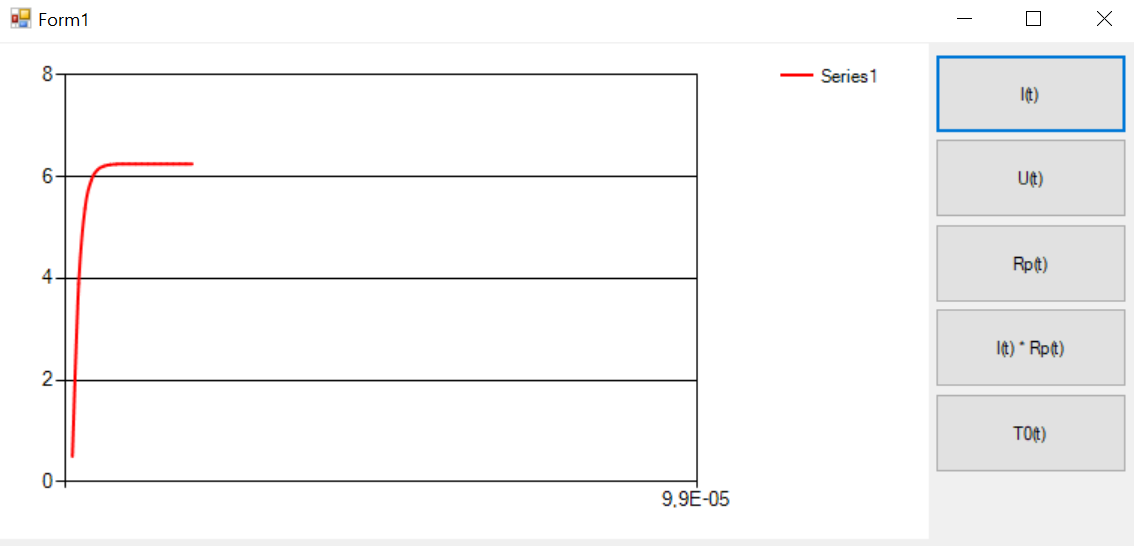
\includegraphics[width=1\linewidth]{img/I(t)Rk200.png}} a) \\
\end{minipage}
\hfill
\begin{minipage}[h]{0.47\linewidth}
\center{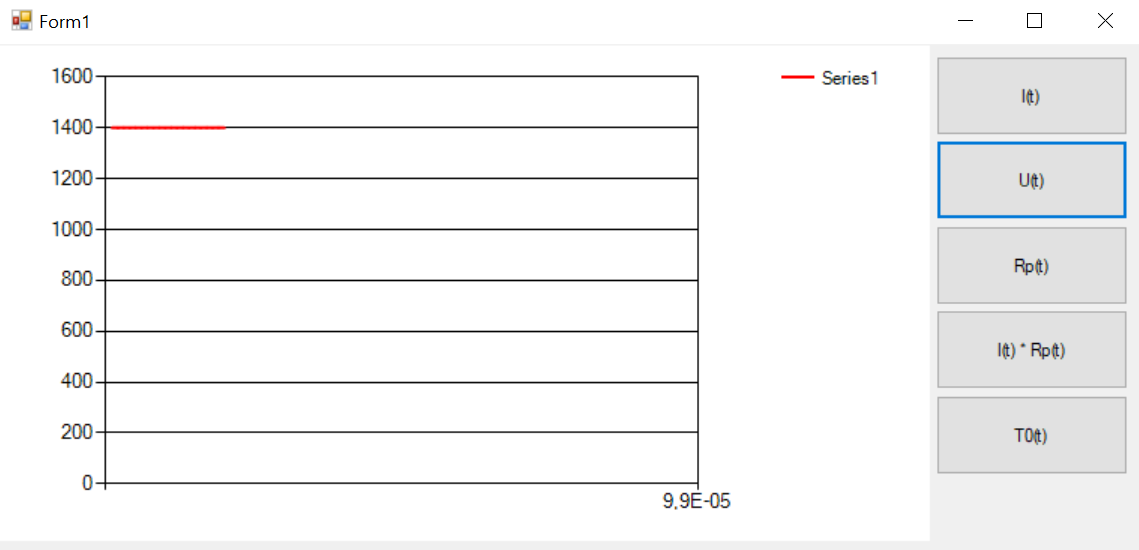
\includegraphics[width=1\linewidth]{img/U(t)Rk200.png}} \\b)
\end{minipage}
\vfill
\begin{minipage}[h]{0.47\linewidth}
\center{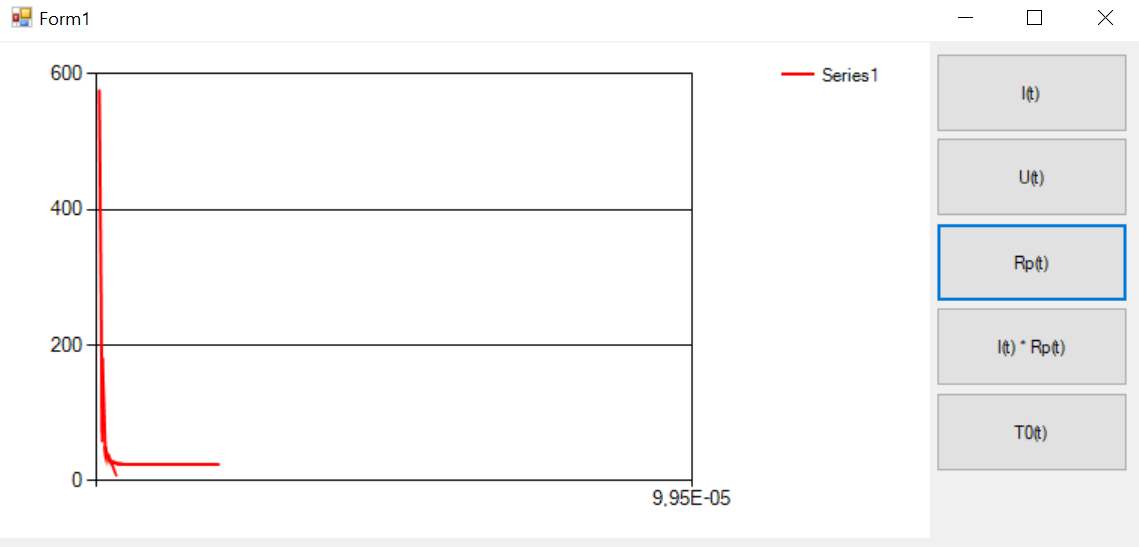
\includegraphics[width=1\linewidth]{img/Rp(t)Rk200.png}} c) \\
\end{minipage}
\hfill
\begin{minipage}[h]{0.47\linewidth}
\center{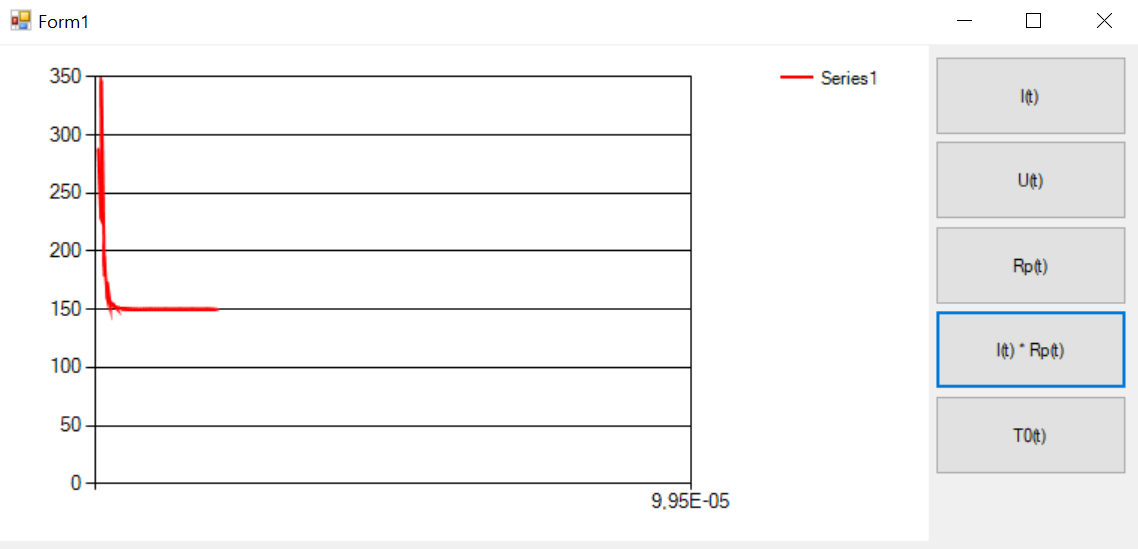
\includegraphics[width=1\linewidth]{img/I(t)Rp(t)Rk200.png}} d) \\
\end{minipage}
\caption{Графики: a) I(t), b)
U(t), c) $R_p(t)$, d) $I(t)*R_p(t)$.}
\label{fig:fig7}
\end{figure}

Результаты исследования влияния параметров контура $C_k, L_k, R_k$ на длительность импульса t имп. апериодической формы.

\begin{figure}[H]
\begin{minipage}[h]{0.47\linewidth}
\center{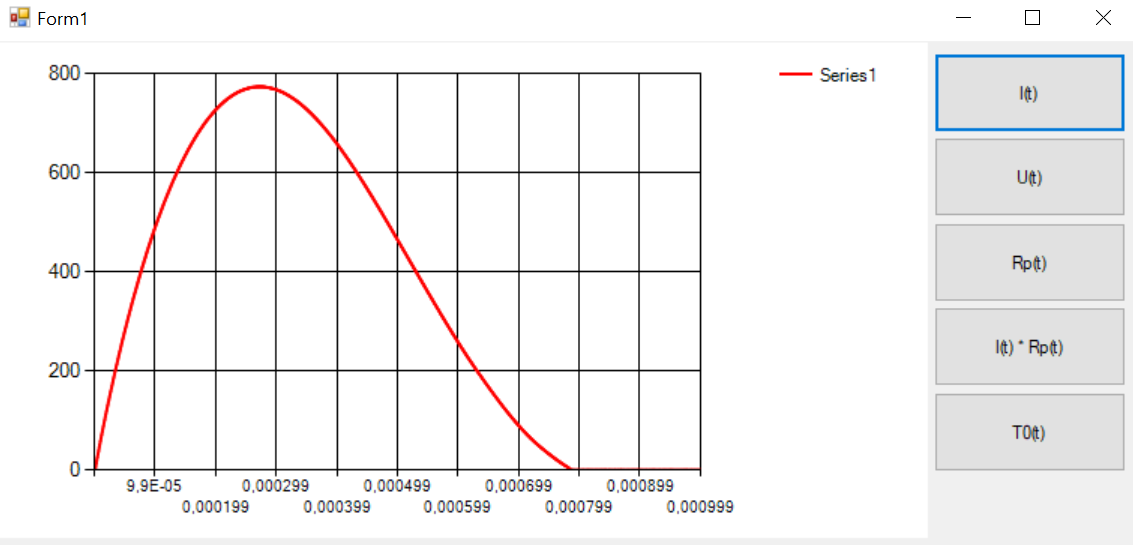
\includegraphics[width=1\linewidth]{img/Ck250.png}} a) \\
\end{minipage}
\hfill
\begin{minipage}[h]{0.47\linewidth}
\center{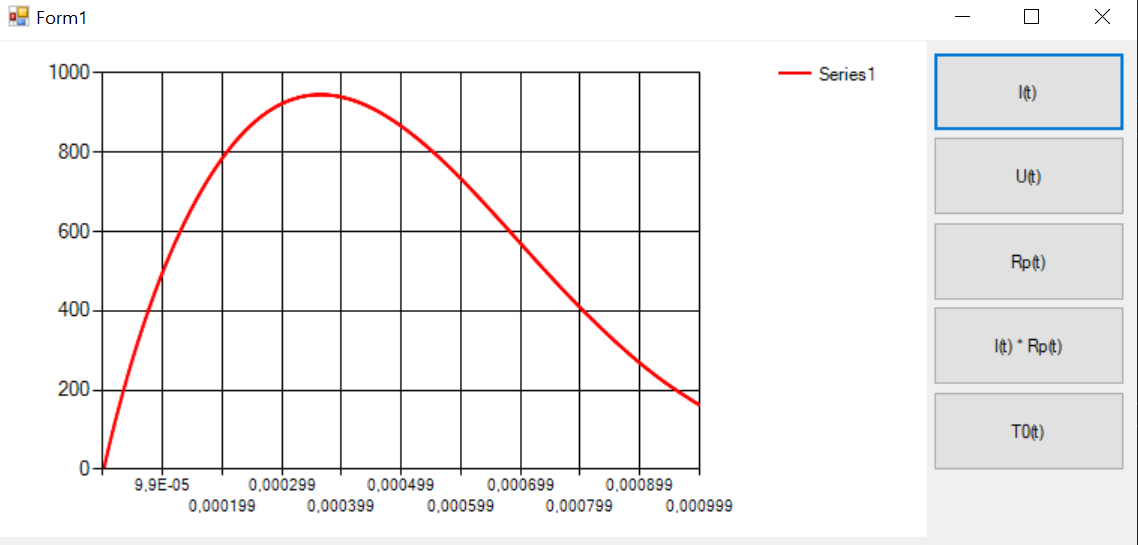
\includegraphics[width=1\linewidth]{img/Ck500.png}} \\b)
\end{minipage}
\caption{Графики: a) $C_k$ = 0,00025, b)
$C_k$ = 0,0005}
\label{fig:fig8}
\end{figure}

a) $C_k$ = 0.000250 $\Delta t$ = 0.000536

b) $C_k$ = 0.000500 $\Delta t$ = 0.000804

При увеличении $С_k$ в 2 раза, $\Delta t$ увеличилось в 1.5 раза


\newpage

\begin{figure}[H]
\begin{minipage}[h]{0.47\linewidth}
\center{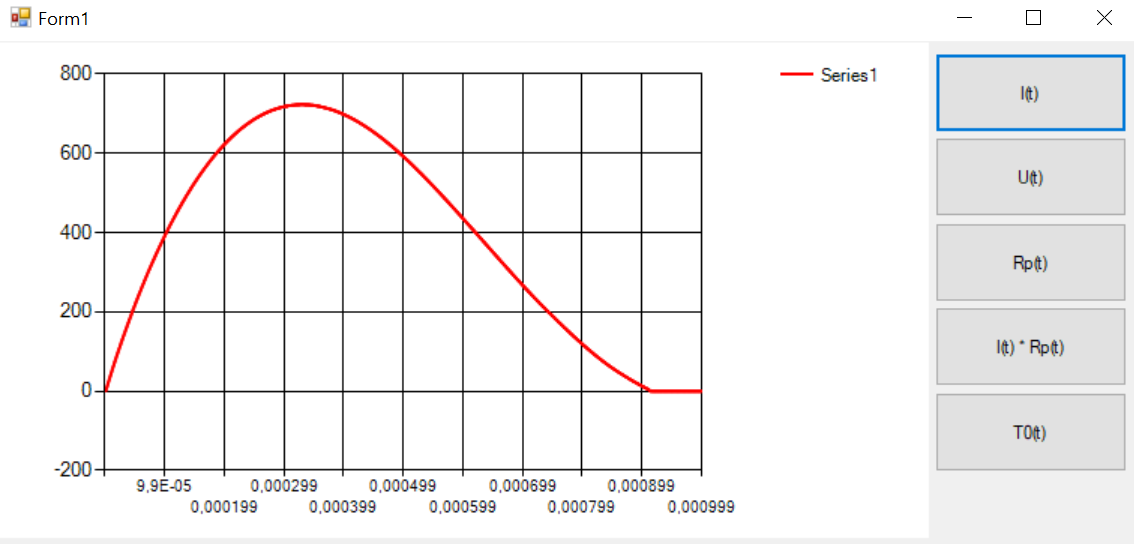
\includegraphics[width=1\linewidth]{img/Lk250.png}} a) \\
\end{minipage}
\hfill
\begin{minipage}[h]{0.47\linewidth}
\center{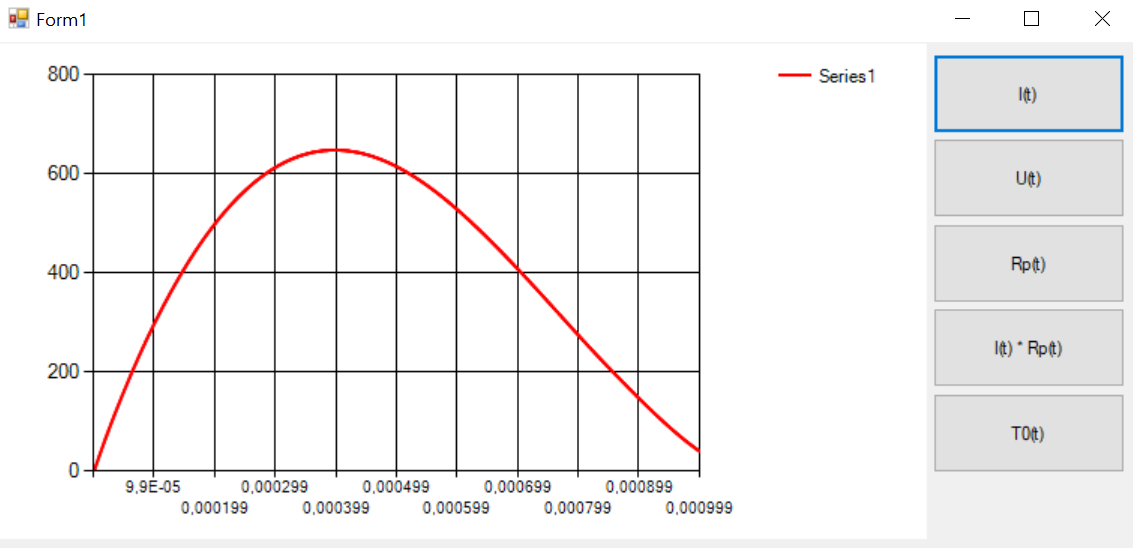
\includegraphics[width=1\linewidth]{img/Lk350.png}} \\b)
\end{minipage}
\caption{Графики: a) $L_k$ = 0.000250, b)
$L_k$ = 0.000350}
\label{fig:fig9}
\end{figure}

a) $L_k$ = 0.000250 $\Delta t$ = 0.000536

b) $L_k$ = 0.000350 $\Delta t$ = 0.000777

При увеличении $L_k$ в 1.4 раза, $\Delta t$ увеличилось в 1.45 раза

\begin{figure}[H]
\begin{minipage}[h]{0.47\linewidth}
\center{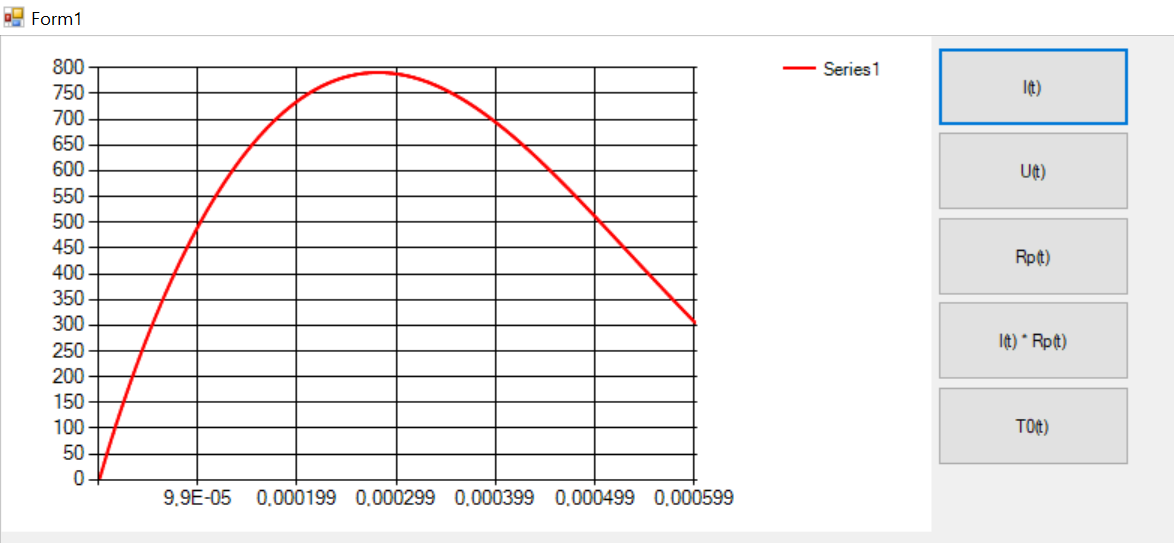
\includegraphics[width=1\linewidth]{img/I(t).png}} a) \\
\end{minipage}
\hfill
\begin{minipage}[h]{0.47\linewidth}
\center{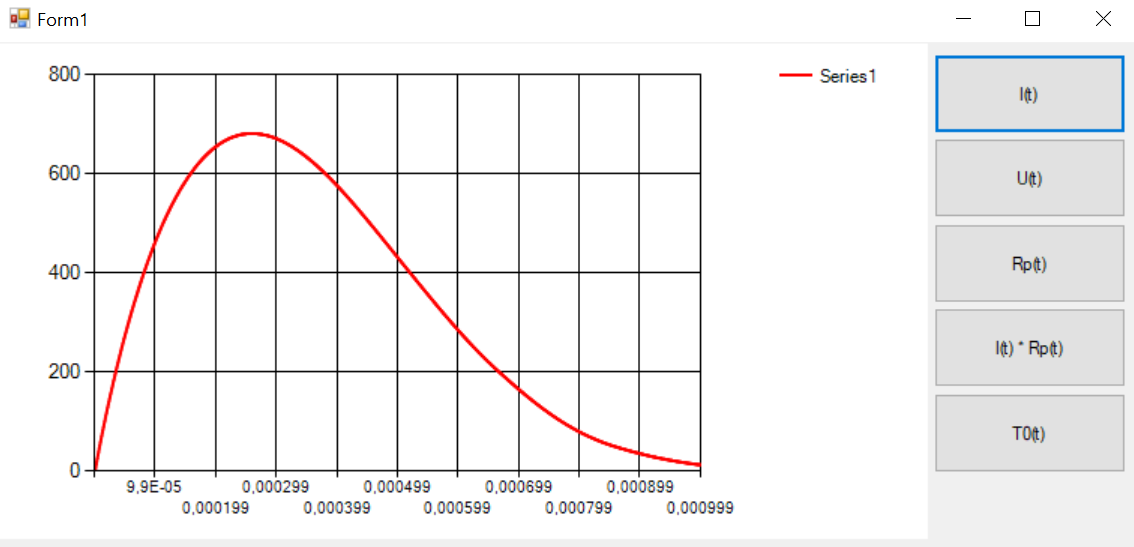
\includegraphics[width=1\linewidth]{img/Rk0.5.png}} \\b)
\end{minipage}
\caption{Графики: a) $R_k$  = 0.25, b)
$R_k$  = 0.5}
\label{fig:fig10}
\end{figure}

$R_k$  = 0.25 $\Delta t$ = 0.000575

$R_k$  = 0.5 $\Delta t$ = 0.000715

При увеличении $R_k$ в 2 раза, $\Delta t$ увеличилось в 1.24 раза



